\chapter{Исследовательская часть}

\section{Среда для тестирования}

Для тестирования разработанного алгоритма применялась облачная платформа Google Colab, не требующая установки ПО на локальный компьютер.

% 

\section{Обучение модели полиномиальной регрессии}

\begin{figure}
	\begin{center}
		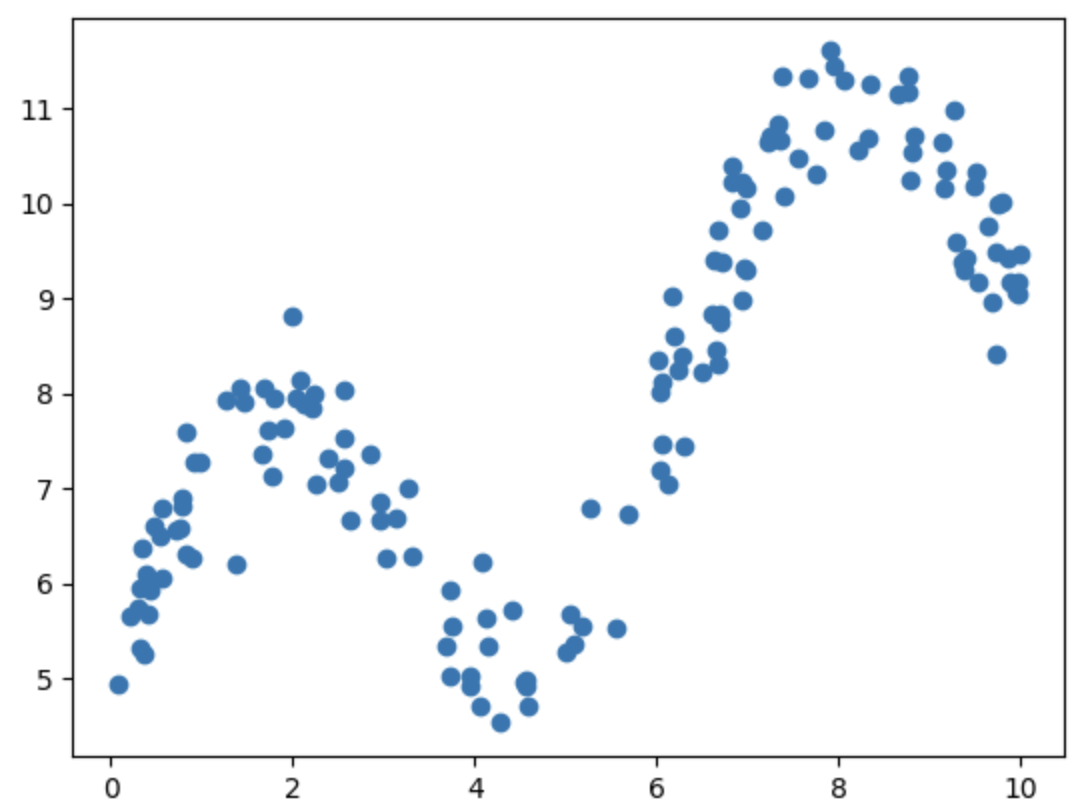
\includegraphics[width=0.75\textwidth]{images/1.png}
	\end{center}
	\caption{Исходные данные}
	\label{img:1}
\end{figure}

\begin{figure}
	\begin{center}
		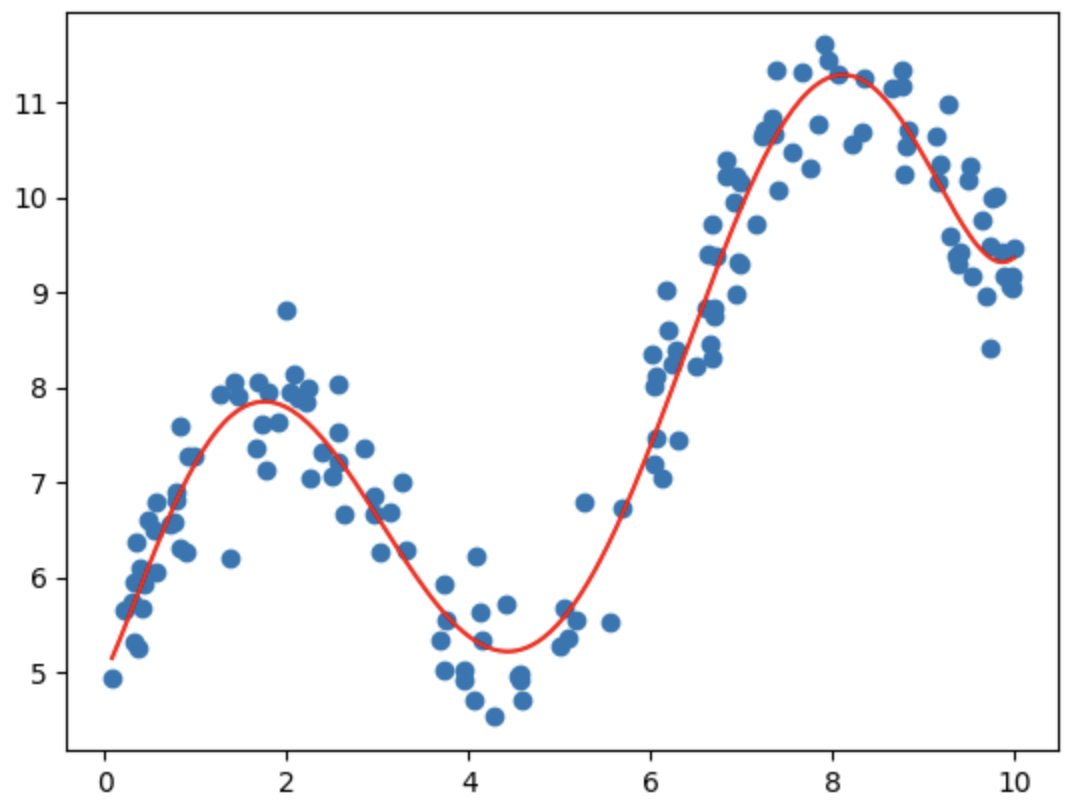
\includegraphics[width=0.75\textwidth]{images/2.png}
	\end{center}
	\caption{Аппроксимация полиномом оптимальной степени (6)}
	\label{img:2}
\end{figure}

\begin{figure}
	\begin{center}
		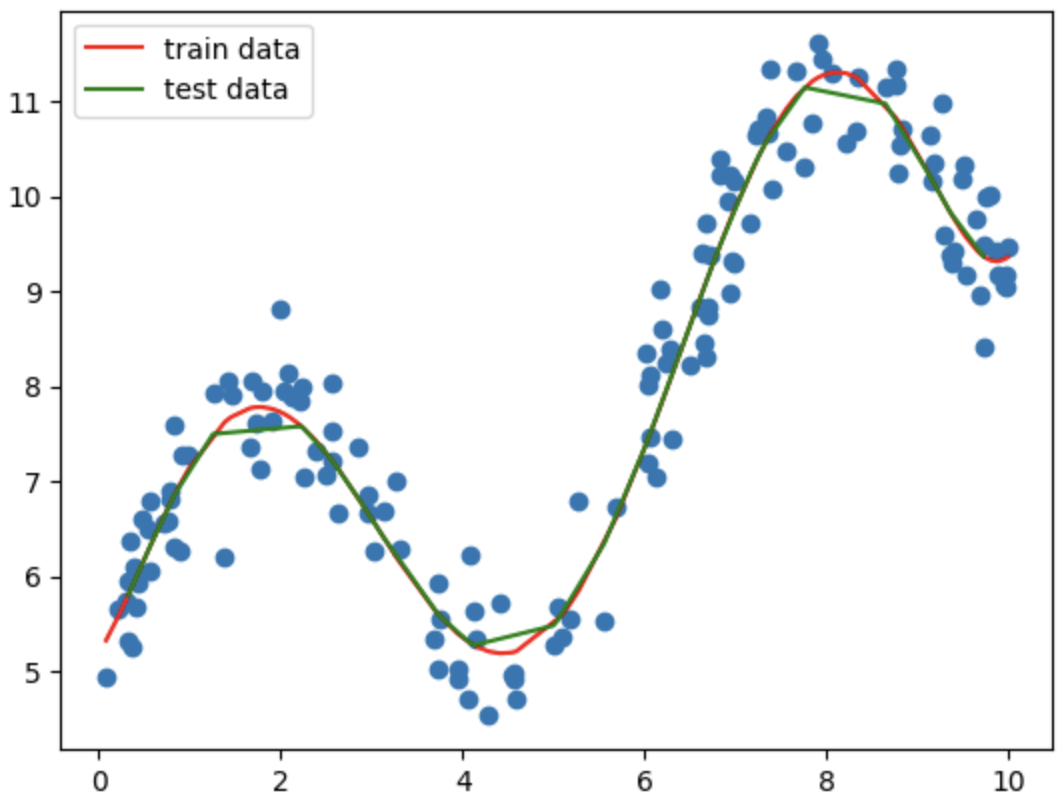
\includegraphics[width=0.75\textwidth]{images/3.png}
	\end{center}
	\caption{Разделение выборки на обучающую и тестовую в отношении 80 на 20}
	\label{img:3}
\end{figure}

\clearpage

\section{Визуализация феномена Рунге}

\begin{figure}
	\begin{center}
		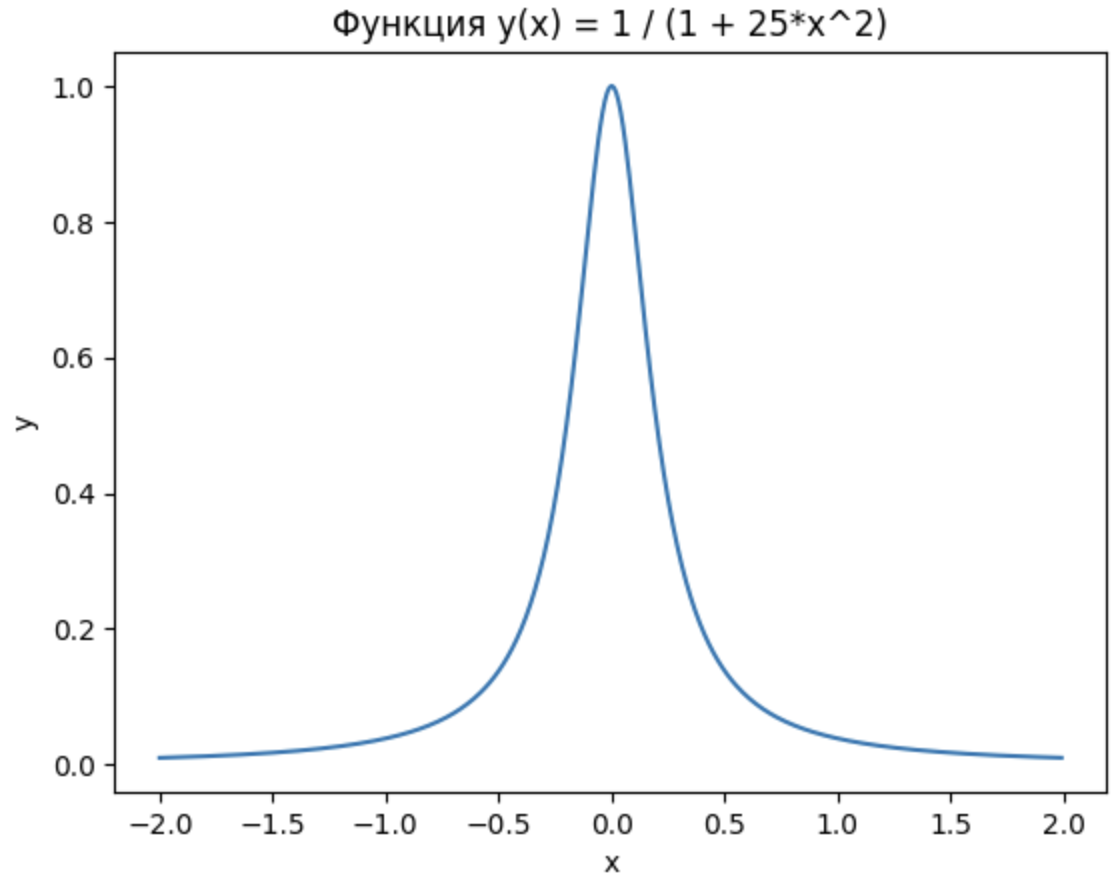
\includegraphics[width=0.75\textwidth]{images/4.png}
	\end{center}
	\caption{Исходные данные}
	\label{img:4}
\end{figure}

\begin{figure}
	\begin{center}
		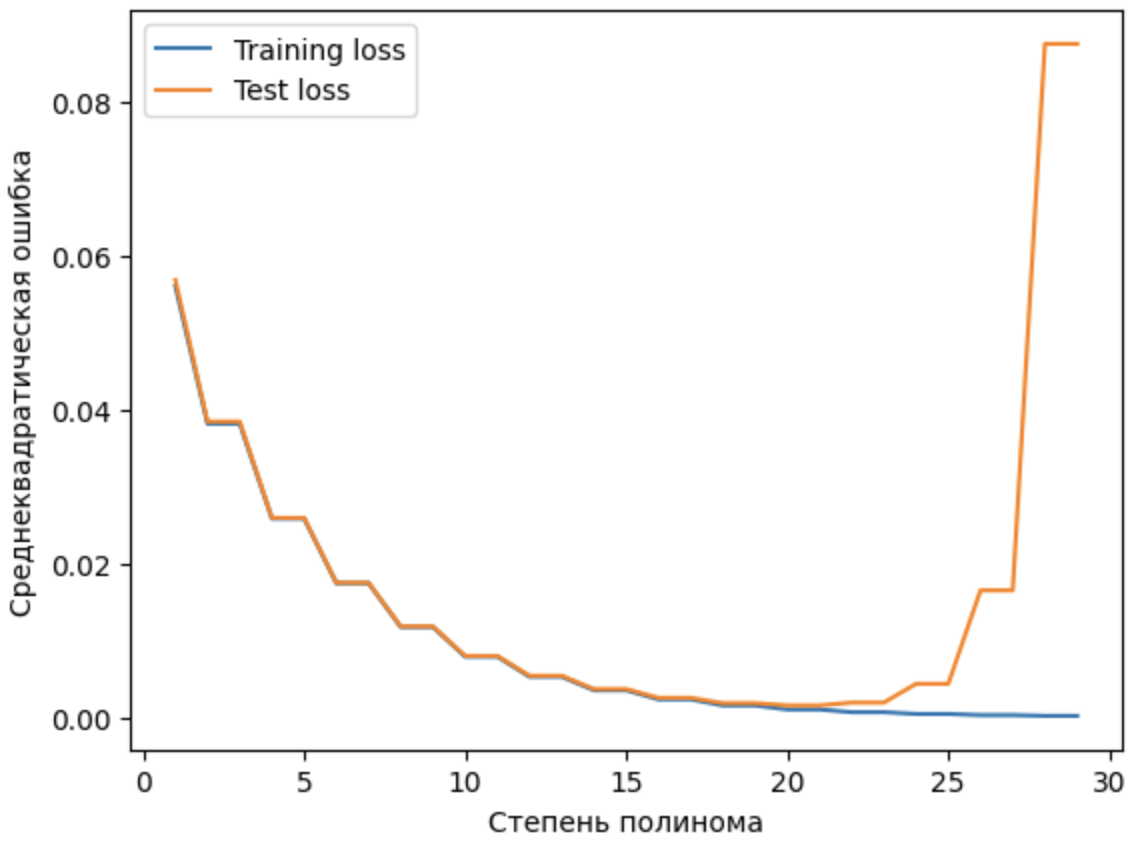
\includegraphics[width=0.75\textwidth]{images/5.png}
	\end{center}
	\caption{Зависимость точности обучения от степени полинома}
	\label{img:5}
\end{figure}

\begin{figure}
	\begin{center}
		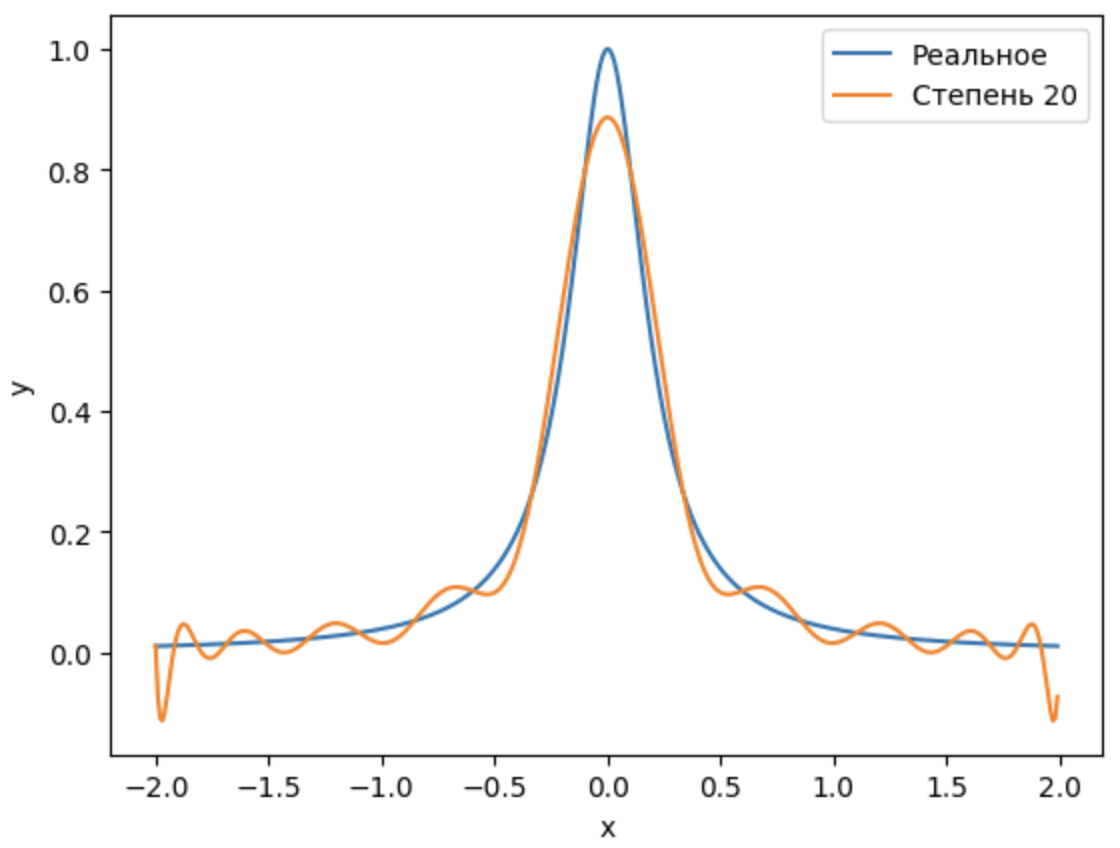
\includegraphics[width=0.75\textwidth]{images/6.png}
	\end{center}
	\caption{Сравнение исходной кривой с полиномом оптимальной степени (20)}
	\label{img:6}
\end{figure}

\begin{figure}
	\begin{center}
		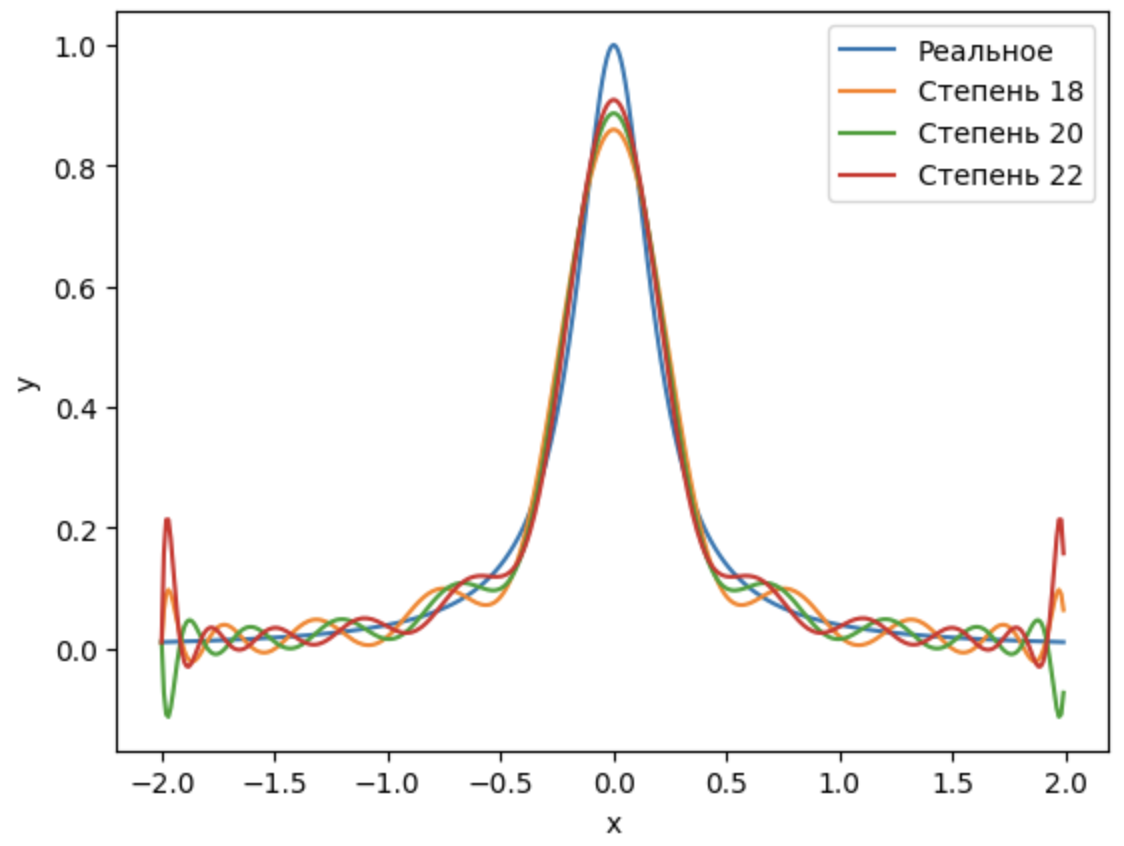
\includegraphics[width=0.75\textwidth]{images/7.png}
	\end{center}
	\caption{Сравнение исходной кривой с полиномами степеней 18, 20 и 22}
	\label{img:7}
\end{figure}

\begin{figure}
	\begin{center}
		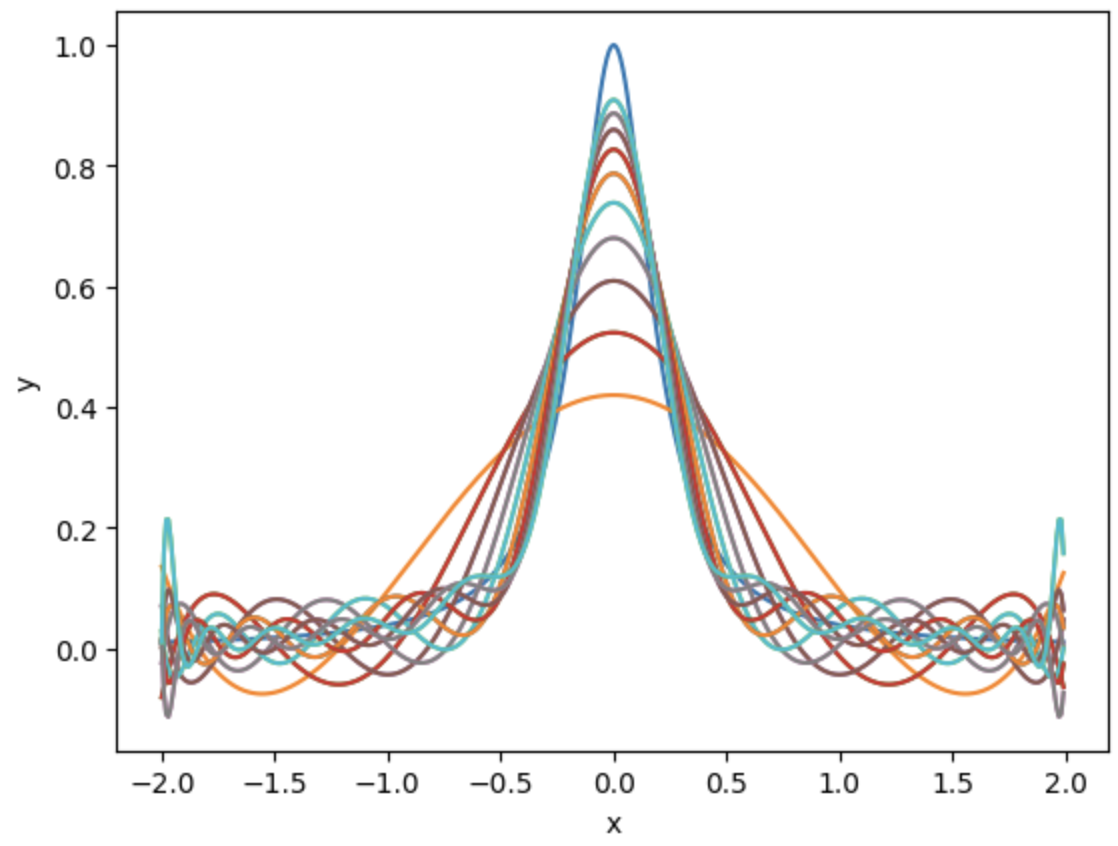
\includegraphics[width=0.75\textwidth]{images/8.png}
	\end{center}
	\caption{Сравнение исходной кривой с полиномами степеней от 5 до 24}
	\label{img:8}
\end{figure}

\begin{figure}
	\begin{center}
		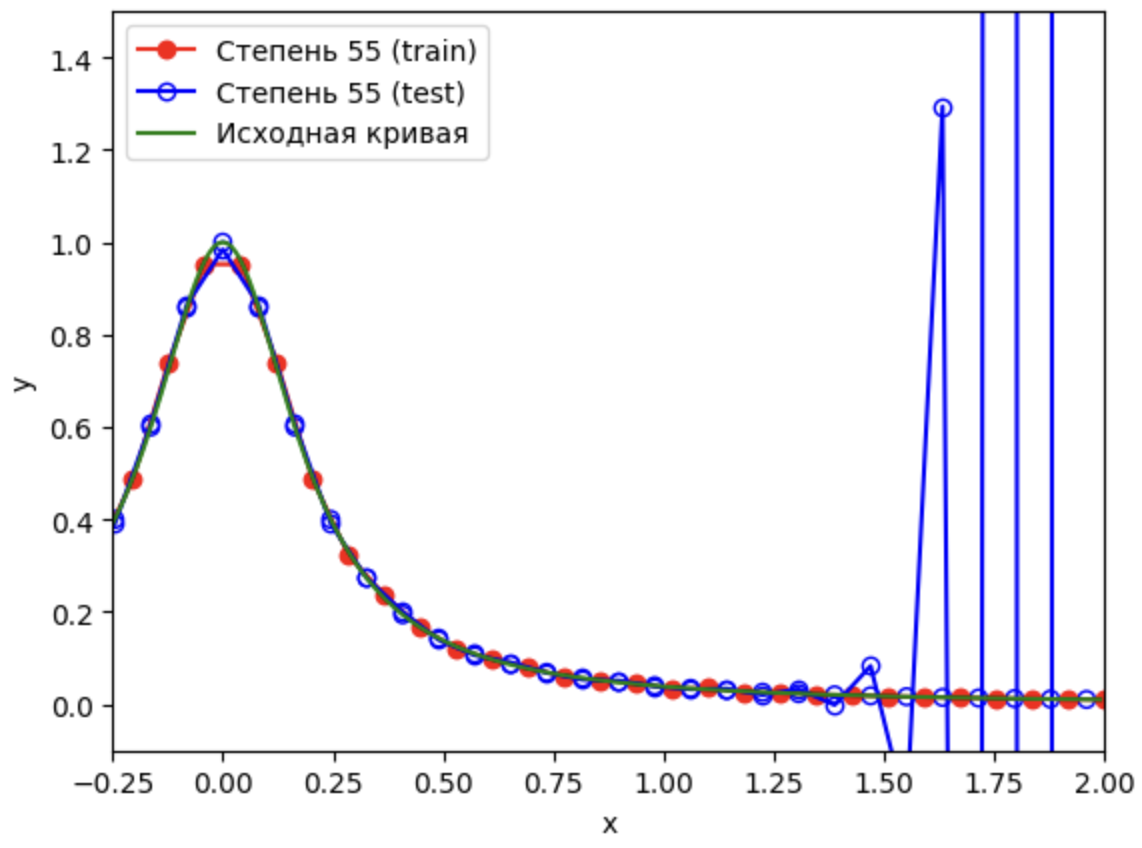
\includegraphics[width=0.75\textwidth]{images/9.png}
	\end{center}
	\caption{Иллюстрация феномена Рунге для исходной кривой, аппроксимированной полиномом степени 55}
	\label{img:9}
\end{figure}

\clearpage
